\chapter{INTRODUCTION}
\label{sec.introduction}
Broadband Internet access for home use is rapidly evolving. The United States
alone has more than 279 million broadband users. The number of Internet 
users in other regions is even more impressive, with China counting more 
than 641 million~\cite{asia}. Yet, despite its pervasiveness, little is 
known about most home networks. This lack of knowledge hampers progress in
a number of important research areas, from ISP performance to large-scale
topology mapping and wireless network utilization. Researchers, policymakers 
and Internet Service Providers (ISPs) are also eager to learn more about 
emerging technologies made possible by these networks. ``Smart homes," in 
which devices from thermostats to door locks can be controlled remotely are
 now exciting realities. In 2016, 4 billion new objects (e.g., laptops, 
handhelds, interactive television, wireless based security cameras) will 
become available to consumers~\cite{gartner}. But with the benefits of these 
products also come concerns. For these devices to work, they usually need to 
be connected to a wireless router. If a router is compromised via buggy 
software, it is possible that hackers could unlock not only critical data, 
but also your front door. Therefore, as their use grows, understanding 
vulnerabilities in both routers and broadband networks becomes crucial in 
order to prevent these types of attacks.

Due to these changes, the value of studying home networks for researchers, 
policy makers and ISPs continues to grow. At this point in time studying 
home networks on a large scale has been difficult because network 
technologies, such as network address translators (NATs), present only an 
opaque view of the home network to the global Internet. To better understand 
the behavior of networks, a formal study using an experimental platform that 
can gather data via from homes  is needed to provide visibility into the 
missing part of Internet. Such a platform should also provide a set of 
programming interfaces to support as wide an array of measurements as 
possible, including factors affecting broadband performance, or data that 
can increase understanding of usage and connectivity in home networks.
Lastly, the ideal platform proposed here should ensure the privacy of the 
user and prevent abuse of his or her device or network resources.

A number of measurement and experimentation platforms have been developed to 
support controlled network experimentation and broadband characterization 
for home networks, including gateway-based platform\cite{bajpai2014lessons,
samknows,183951,yiakoumis2014behop} and browser or host-based platform\cite{
dhawan2012fathom,kreibich2010netalyzr,sanchez2014measurement}. Host-based 
platforms run as applications on the client side and typically suffer from a 
few limitations (e.g., reflecting the network performance of the host or 
application rather than of the network itself, providing only one-shot 
measurements rather than continuous measurements). A gateway-based platform 
on the other hand, enables continuous measurements and collect network 
feedback from all the WiFi devices in the home networks. However, these 
platforms could not balance the trade-off between functionality and security.
 For instance, the process of vetting BISmark~\cite{183951} experiments for 
researchers is manual, which will be a limiting factor a deployment grows. 
Inspired by these projects, we decided to design a gateway-based platform 
that enables continuous, comprehensive and direct measurements. We also 
designed the platform with user security and privacy as a first-order concern.
 
In this paper, we introduce \sysname, a distributed cloud platform that 
allows researchers to run both active and passive experiments securely from 
a wireless router on a home network. Through a programmable interface on the 
device, the platform enables researchers to deploy a wide range of network 
measurements from a vantage point between the access ISP and the home 
network, as shown in Figure~\ref{figure:design}. Researchers can access and 
compile data on systems worldwide, while preserving the user's privacy, and 
securing the device itself. The information gathered from such studies could 
assist users in evaluating the services they are paying for, researchers in 
understanding the factors impacting performance, and ISPs in finding ways to 
improve their service. \sysname implements a number of measurement 
primitives to enable researchers, policy makers and Internet Service 
Providers (ISPs) to program network measurements. To protect device 
availability and privacy, \sysname supports a very flexible language for 
experiment specification based on Repy, a lightweight, Python based, 
performance isolation and extensible programming language~\cite{
cappos2010retaining}. Because it is designed for running measurement 
software on a home access point, a platform like \sysname has a number of 
unique strengths and challenges. First, software must be small and easy-to-
deploy because \sysname is deployed on resource-constrained devices. Second, 
\sysname sits on the direct path of real Internet users. Any buggy or 
malicious experiments could be able to disrupt Internet connectivity. Thus 
it must guarantee that a poorly designed experiment can not negatively 
effect a user's Internet connection. Third, it is important to make the 
system robust by providing remote maintenance and updates because of the 
unmanaged complexity of its home network environments. Finally, \sysname 
must provide a rich set of APIs for a variety of network measurements. 

\begin{figure}%[h]
\centering
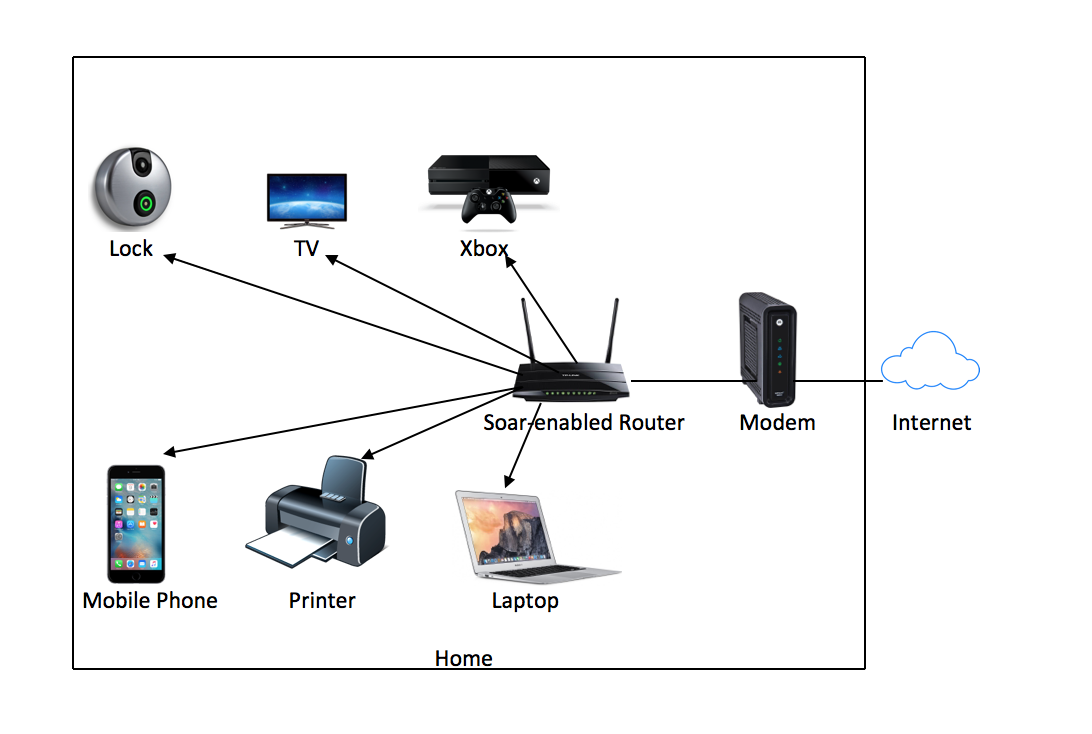
\includegraphics[width=0.8\columnwidth]{figure/home-network.png}
\caption{The SOAR-enabled router sits on the direct path of real 
Internet users. It supports both active and passive network measurements.}
\label{figure:design}
\end{figure}

The primary contributions of this study are as follows:
{\raggedright
\begin{itemize}
\item\textbf{1) Home routers platform deployment:} This platform is based on Seattle testbed, a community-driven and open-source cloud computing system~\cite{zhuang2013experience,cappos2009seattle}. Compared to computer and mobile device environments, deployment on home wireless router has more resource limitation such as restricted computational resources. However, recently we are able to port Seattle Testbed to OpenWrt, a popular Linux platform for home routers~\cite{openwrt}. Users can build their own \sysname installer (IPK) via config file we provide using OpenWrt SDK and install it on the device directly. 

\item\textbf{2) Extensions to Seattle Testbed:} Our testbed implements new research capabilities for home wireless router by improving on the Seattle sandbox. To handle home wireless routers, our testbed uses low-level system calls in the OpenWrt platform with the Restriction Python (Repy)~\cite{cappos2010retaining}, the core sandbox of Seattle. In order to securely interact with home routers on remote user devices, we use Fence (a non-intrusive mechanism that mediates and limits access to diverse resources using uniform resource control)~\cite{li2015fence} to allocate a fixed percentage of the device's CPU, memory disk, and other resources to one or more VMs. For example, we set the legal times of accessing \emph{/proc} file system to prevent DoS attack using our API calls. Our testbed adds eight functionalities based on Repy, include \texttt{get\_network\_bytes}, \texttt{get\_network\_packets}, \texttt{get\_network\_interface}, \texttt{wifi\_status}, \texttt{scan}, \texttt{get\_station}, \texttt{ping} and \texttt{traceroute}. These rich set of measurement primitives help researchers to implement a wide range of network measurements, such as mapping Internet paths (via traceroute), studying home network usage pattern and understanding wireless network performance.

\item\textbf{3) Experimental characterization of home wireless networks:} By integrating \sysname into the home networks, we get the benefits of a real world deployment while ensuring flexibility to run experiments without compromising home network. We demonstrate \sysname's utility by implementing hybrid measurements that together exercise different new API calls (e.g, \texttt{get\_network\_bytes}, \texttt{get\_network\_interface}, \texttt{wifi\_status}): Characterizing home wireless performance from gateway view. We monitor our lab's network traffic, which in an office building, from the vantage point of the gateway. We report on additional experiences gained using \sysname in three different use cases. We find that there are many factors affecting throughput on 2.4 GHz and 5 GHz band. We also find that most of access points select non-overlapping channels (e.g., channel 1, 6, 11) to avoid adjacent-channel interference. 
\end{itemize}
\par}
The rest of thesis is structured as follows: We provide related works and motivation in \S{\ref{sec.relatedwork_motivation}}. In \S{\ref{sec.goals_challenges}}, we point out the goals and challenges of our work. \S{\ref{sec.design}} and \S{\ref{sec.implementation}} describes the design and implementation of \sysname and characterize our current deployment. Then we present three study cases to illustrate the benefits of an experimental platform that runs on the home wireless router in \S{\ref{sec.evaluation}}. Finally, we discuss future work and conclusion in \S{\ref{sec.conclusion}}. 